\documentclass[a4paper,11pt,twoside,table,xcdraw]{article}
%\documentclass[a4paper,11pt,twoside,se]{article}

\usepackage{UmUStudentReport}
\usepackage{verbatim}   % Multi-line comments using \begin{comment}
\usepackage{courier}    % Nicer fonts are used. (not necessary)
\usepackage{pslatex}    % Also nicer fonts. (not necessary)
\usepackage[pdftex]{graphicx}   % allows including pdf figures
\usepackage{listings}
\usepackage{pgf-umlcd}
\usepackage{blindtext}
\usepackage{enumitem}
\usepackage{amsmath}
\usepackage{amssymb}
%\usepackage[table,xcdraw]{xcolor}
%\usepackage{lmodern}   % Optional fonts. (not necessary)
%\usepackage{tabularx}
%\usepackage{microtype} % Provides some typographic improvements over default settings
%\usepackage{placeins}  % For aligning images with \FloatBarrier
%\usepackage{booktabs}  % For nice-looking tables
%\usepackage{titlesec}  % More granular control of sections.

% DOCUMENT INFO
% =============
\department{Department of Computing Science}
\coursename{Parallel Programming 7.5 p}
\coursecode{5DV152}
\title{Final Programming Assignment\\ MPI Game of Life}
\author{Lorenz Gerber ({\tt{dv15lgr@cs.umu.se}} {\tt{lozger03@student.umu.se}})}
\date{2017-03-26}
%\revisiondate{2016-01-18}
\instructor{Lars Karlsson / Mikael Ränner}


% DOCUMENT SETTINGS
% =================
\bibliographystyle{plain}
%\bibliographystyle{ieee}
\pagestyle{fancy}
\raggedbottom
\setcounter{secnumdepth}{2}
\setcounter{tocdepth}{2}
%\graphicspath{{images/}}   %Path for images

\usepackage{float}
\floatstyle{ruled}
\newfloat{listing}{thp}{lop}
\floatname{listing}{Listing}



% DEFINES
% =======
%\newcommand{\mycommand}{<latex code>}

% DOCUMENT
% ========
\begin{document}
\lstset{language=C}
\maketitle
\thispagestyle{empty}
\newpage
\tableofcontents
\thispagestyle{empty}
\newpage

\clearpage
\pagenumbering{arabic}

\section{Introduction}
Here it was the aim to design and implement conway's game of life that can be run on a High Performance Computing system using the MPI library. 
\section{Conway's Game of Life}
Conway simplified mathematical models from von Neuman that were about structures which had the ability to copy themselves. Published 1970, the surprising property of the program was that it represented a Turing complete system despite using only very few simple rules. It was the start of a new research field about `cellular automata'.

Conway's game of life is represented by a regular grid of limited size that consists of individual cells which can either be death or alive. The game of life proceeds in rounds: In each round the state of each cell is evaluated individually and then updated to an eventual new state. The most important feature of this system are the rules applied for assessing and updating the state of each individual cell: Based on the eight neighboring cells, it is determined if a cells environment is life promoting or overcrowded. Hence, the variable to determine and evaluate is the number of neighboring cells alive.

\section{Design and Implementation}
From the description of the game itself, some preliminary design drafts were sketched. Then a short literature study about available implementations was conducted. Several programs of interest were found and inspected for inspiration \cite{golRosetta} \cite{golKTH} \cite{golPetascale}. 
To be flexible, it was decided to implement both randomized game start state and loading of a saved state from file. Because graphics programming was not the focus of this course a simple script in R \cite{rlanguage} was written for visual inspection of the game state after a number of generations. 
`Foster's Methodology' as reproduced in the course literature \cite[p. 66]{pacheco2011} was applied for designing the parallel program:

\begin{enumerate}
\item Partitioning\\
Two task were identified: Detecting the number of neighbors alive and updating the state for the next round. However, as it will be seen later, in the current case, it could make more sense to see the operations of each single cell as an individual task.
\item Communication\\
The two first mentioned tasks above need to run in sequence and they also need to be concerted among the whole game. If a single cell is seen as an individual task, then the communication would be the step where the state of the neighboring cells is determined. The cell is locally dependent to access the eight surrounding cells. 
\item Agglomeration / Aggregation\\
Agglomerating the individual tasks per cell seems to make sense as they adhere to a strict temporal run sequence. However more interesting is to consider agglomerating larger numbers of individual cells. As most of the cells would have eight neighbors within the group, they could be considered to be independent with a few exceptions for the cells on the interface/border. 
\item Mapping\\
As the identified tasks are tightly coupled, it seems to make most sense to map larger agglomerates of cells to individual MPI nodes. Hence, communication during the game will be limited to handling the mentioned special cases of cells that are at the border of a local cell group. 
\end{enumerate}

For the implementation it was decided to divide the global square field along vertical lines into equal sized local rectangular fields. As such, communication between nodes included only the cells that were on the vertical borders as the horizontal borders (top and bottom) could be accessed locally. To facilitate communication, the local rectangular cell groups were padded with one layer of cells where the cell state from the next-by local border could be imported to.

This strategy resulted in a total of three tasks per game cycle:
\begin{enumerate}
\item update interface region
\item determine number of neighbors alive
\item update state
\end{enumerate}



\section{Usage Instructions}
\subsection{Building}
The makefile that builds both the serial (\verb+serial_life+) and MPI parallel version (\verb+mpi_life+) is provided. In the HPC2N environment, the user only needs to load the appropriate compiler module (eg \verb+module load openmpi/gcc/1.8.8+), go to the directory with the source code and run \verb+make+. \verb+make clean+ was configured to clean up the directory from \verb+.o+, \verb+.txt+ and \verb+.pdf+ files. 

\subsection{Usage}

\subsubsection{Running the Program}
Both the serial and the parallel version use the same simple command argument parser that accepts either three or four command line arguments. These are in sequence: \verb+n_size+ \verb+generations+ \verb+outfile+ \verb+[infile]+. If no infile is indicated, a random start state for the simulation is created. The only output to stdout obtained from the programs is the runtime. However, a file with the game field as a text file is written to the working directory using the filename indicated as command line argument.
\subsubsection{Graph Output using R Script}
To obtain graphical output a short R script was written. Hence to obtain a graphical result it is needed to have the R language interpreter installed on the system \cite{rlanguage}. The script shown below can be run from the command line with the following command:\\
\verb+Rscript --vanilla plot_Script.R data_file.txt graphical_output.pdf+\\
This command will use the output from either \verb+serial_life+ or \verb+mpi_life+ (\verb+data_file.txt+) and render the pdf file \verb+graphical_output.pdf+.   
\begin{verbatim}
#!/usr/bin/env Rscript
args = commandArgs(trailingOnly=TRUE)

# test if there is at least one argument: if not, return an error
if (length(args)==0) {
  stop("At least one argument must be supplied (input file).n", call.=FALSE)
} else if (length(args)==1) {
  # default output file
  args[2] = "life_image.pdf"
}

## preparing data
data<-read.csv(file=args[1], sep=" ", header=FALSE)
image_data<-matrix(data[1,1]*data[1,2], data[1,1], data[1,2])

for(i in 2:dim(data)[1]){
  image_data[data[i,1], data[i,2]] <- 1
}

# plotting to file
pdf(file = args[2])
image(image_data, main="Conway's Game of Life", 
        xaxt='n', yaxt='n', ylab=paste("y size: ", 
        data[1,2]), xlab=paste("x size: ", data[1,1]))
dev.off()
\end{verbatim}

\section{Validation}
Here the qualitative result of the serial and parallel version were evaluated to yield the same result. This was done using a bash script that runs both programs and then compares the output files using the system tool diff. Two versions of the bash script are contained in the source folder: \verb+validation.sh+ can be used on a shared-memory desktop system without batch submission. \verb+validation_hpc2n.sh+ can be submitted on the HPC2N `Abisko' cluster system using \verb+sbatch ./validation_hpc2n.sh+. This script includes currently the student account that was assigned to the user `stud02'.

The typical output of a validation session is shown below:
\begin{verbatim}
Generating random 1024 x 1024 game field
running serial implementation on random data (100 generations)...
running mpi implementation using 4 processes on random data (100 generations)...
comparing the resulting datasets...
No output from 'diff', validation succeeded
\end{verbatim}

\section{Benchmarking}
Initially, a run to compare the serial with the the MPI implementation running on a single process was performed. A square game of size $n=1000$ with the same start state was run in 1000 generations with each 3 replicates. Both implementations resulted in low variation within and minimal difference between the two implementations (data not shown). Hence, for benchmarking it was decided to only use the MPI version.

The mpi implementation was run on the HPC2N `Abisko' cluster. All timing runs included 100 game generations. MPI runs where conducted with $k={1, 2, 4, 8, 16}$ processes. From preliminary evaluation of the data using boxplots in R \cite{rlanguage} (plots not shown) it was obvious that the variance per replication (3 technical replicates) was very low compared to the total run time. Hence it was decided to calculate median values without presenting a measure of variation for each configuration. A graphical summary of the benchmarking is shown in figure \ref{fig:global}. 

\begin{figure}
  \centering
  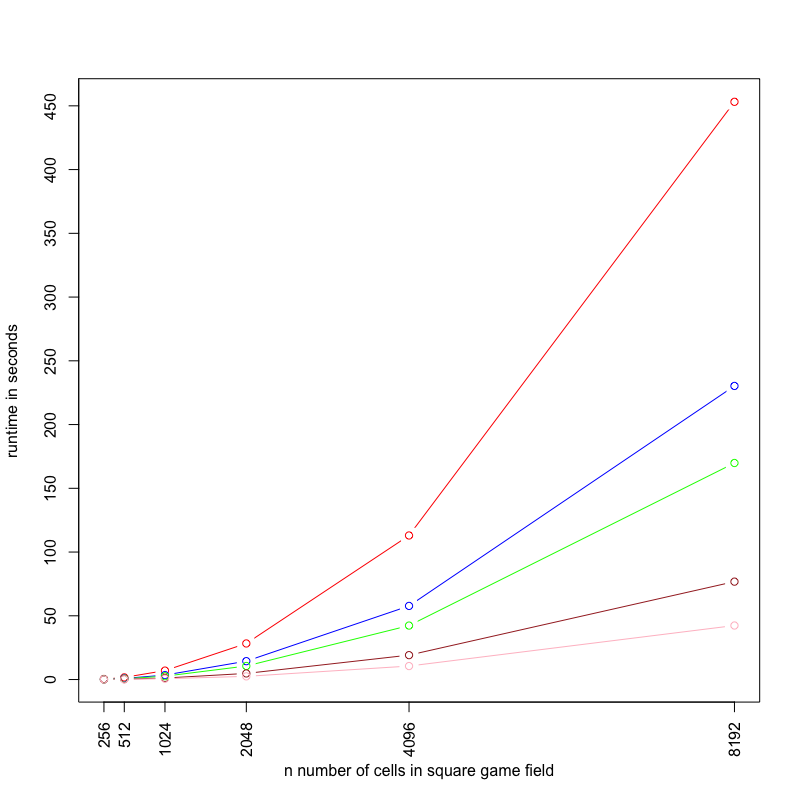
\includegraphics[width=1\textwidth]{global.png}
  \caption{\textit{This figure shows the whole benchmarking data aggregated per core and field size using the median}}
  \label{fig:global}
\end{figure}

Table \ref{tab:result} shows a detailed numerical evaluation with obtained speedups ($S$), efficiencies ($E$) and absolute parallel overheads ($O$) for all configurations. Looking at the data, it sticks directly out that running two MPI processes obtained ideal speedups and efficiencies around 1 while for four MPI processes speedups and efficiencies dropped significantly. For higher even higher number of MPI processes two effects can be observed: At smaller game sizes, speedups are modest and efficiencies even drop. At larger game sizes, speedups get somewhat better again and efficiencies sometimes slightly increase or at least stay at the same level. The sharp break between two and four processes could partly be due to the intrinsic fact that the number of neighbors each process corresponds with increases here: Two processes always communicate only with 1 additional neighbor as the game field folds over in both directions. For three and more processes, each process communicates always with two other processes.


\begin{table}[]
\centering
\caption{\textit{The table below shows a detailed numerical evaluation of the benchmarking with speedups (S), efficiencies (E) and absolute parallel overhead times (O) for all configurations. Each configuration was measured in triplicates.}}
\label{tab:result}
\begin{tabular}{
>{\columncolor[HTML]{C0C0C0}}l 
>{\columncolor[HTML]{EFEFEF}}l |cccc}
\cellcolor[HTML]{EFEFEF}       &   & \multicolumn{4}{c|}{\cellcolor[HTML]{C0C0C0}number of MPI processes}                                           \\
\cellcolor[HTML]{EFEFEF}n size &   & \cellcolor[HTML]{EFEFEF}2 & \cellcolor[HTML]{EFEFEF}4 & \cellcolor[HTML]{EFEFEF}8 & \cellcolor[HTML]{EFEFEF}16 \\ \hline
256                            & S & 1.98                      & 2.57                      & 4.56                      & 6.62                       \\
                               & E & 0.99                      & 0.64                      & 0.57                      & 0.41                       \\
                               & O & 0.00                      & 0.06                      & 0.04                      & 0.04                       \\ \hline
512                            & S & 1.95                      & 2.59                      & 5.43                      & 9.48                       \\
                               & E & 0.98                      & 0.65                      & 0.68                      & 0.59                       \\
                               & O & 0.02                      & 0.23                      & 0.10                      & 0.07                       \\ \hline
1024                           & S & 2.01                      & 2.67                      & 5.94                      & 11.03                      \\
                               & E & 1.00                      & 0.67                      & 0.74                      & 0.69                       \\
                               & O & -0.01                     & 0.87                      & 0.30                      & 0.20                       \\ \hline
2048                           & S & 1.96                      & 2.67                      & 5.91                      & 11.33                      \\
                               & E & 0.98                      & 0.67                      & 0.74                      & 0.71                       \\
                               & O & 0.27                      & 3.53                      & 1.25                      & 0.73                       \\ \hline
4096                           & S & 1.96                      & 2.67                      & 5.90                      & 10.68                      \\
                               & E & 0.98                      & 0.67                      & 0.74                      & 0.67                       \\
                               & O & 1.24                      & 14.08                     & 5.02                      & 3.52                       \\ \hline
8192                           & S & 1.97                      & 2.67                      & 5.90                      & 10.69                      \\
                               & E & 0.98                      & 0.67                      & 0.74                      & 0.67                       \\
                               & O & 3.72                      & 56.57                     & 20.15                     & 14.06                      \\ \hline
\end{tabular}

\end{table}


Probably the degradation of speedups and efficiencies for larger number of processes is due to the very tight temporal synchronization of the game: It probably happens regularly that processes have to wait for each other due to the send/receives which are currently coded as individual events. Probably, some performance increase would be possible if one would change this communication to a collective communication strategy.

However, when looking at the absolute parallel overhead times it can also be seen that they decrease with increasing size of the game field. This is a good sign and suggests that the application is at least weakly scalable in regard of the game field size. This would however not hold true for increasing the problem size by the number of generations to be calculated.



\addcontentsline{toc}{section}{\refname}
\bibliography{references}

\end{document}
